\section{Missions}
\label{missions}
Le moyen de présenter les concepts retenus est une approche par missions. Cette approche a été choisie sur base de l'analyse des autres initiatives similaires dans le chapitre \ref{travail associé}. Dans le cadre de ce travail, une série de missions ont été produites pour avoir une plateforme utilisable.

Après l'explication du schéma général des missions, une description de chacune des quatre missions est présentée ainsi que les concepts qu'elles apportent.

\subsection{Schéma général}
Une fois le choix de l'approche par mission fait, il a fallu définir comment amener la théorie de la programmation à travers ces missions. Il s'est avéré que pour capter l'attention et l'intérêt des étudiants, il était nécessaire qu'elles aient un but final. Chaque mission réussie mène à la mission suivante et introduit de nouveaux concepts de programmation. La dernière mission intègre les différents concepts à travers un jeu de poursuite. Dans ce jeu, un chien doit courir après un chat et le manger. Cet objectif ludique permet d'introduire plusieurs concepts de programmation intéressants tels que la succession d'instructions, les conditions, les boucles, les événements \ldots

Les missions ont donc été conçues dans le but de pouvoir réaliser ce jeu, ce qui met l'accent d'avantage sur la réalisation d'un jeu que sur l'apprentissage de concepts. Dans cette optique, les concepts nécessaires à la réalisation de la mission chien et chat sont introduit dans 3 pré-mission. L'introduction progressive des concepts permet de se concentrer sur un à deux grand concept par mission. Ceci diminue les introductions théorique des missions et augmente les temps ou les enfants crées les programme.

La chronologie des missions est pensée pour avoir une progression. La première introduit la programmation impérative, la seconde amène les boucles et la troisième donne l'intuition de la programmation événementielle. La dernière mission réutilise tous ces concepts.

Les trois pré-missions sont : la voiture, l'hélicoptère et soyons courtois.


% Une fois le choix de l'approche par mission choisi, il faut définir comment amener la théorie de la programmation à travers ces missions. Il s'est avéré que pour capter l'attention et l'intérêt des étudiants, il était nécessaire d'introduire les missions par la présentation d'un but final. Celui retenu dans ce travail a été le jeu du chien et du chat. Dans ce jeu le chien doit courir après le chat et le manger. Le principe de ce jeu est très simple et permet l'introduction de plusieurs concepts de programmation intéressants tels que la condition, les boucles et également les événements.\\
% 
% Pour introduire les concepts de manière douce, la mission finale \texttt{Chien et chat} est introduite par trois missions d'introduction : \texttt{la voiture}, \texttt{l'hélicoptère} et \texttt{Soyons courtois}. Dans la suite de cette partie, nous allons décrire les missions et faire une analyse des concepts introduits.

\subsection{Voiture}
\label{mission-voiture}
Dans cette première mission, voir figure \ref{fig:mission-voiture}, les participants sont mis dans un bolide qui doit atteindre la ligne d'arrivée en restant sur la route. Si la voiture sort de la route, elle explose. À chaque lancement du script la voiture reprend sa position d'origine.\\

Cette mission vise à ce que les participants puissent prendre en main l'interface de Snap! et à introduire la notion de suite d'instructions. Ils devaient enchaîner des blocs de déplacement dans lesquelles, le nombre de pas ou l'angle de virage étaient à compléter.

Le fait de devoir prévoir les instructions n'est pas un concept facile pour le public cible. Beaucoup exécutent une opération et puis cherchent à savoir comment continuer à partir de leur nouvelle position. Dans cette mission, la voiture retournant à chaque fois à son point de départ, les élèves sont forcés à réfléchir de manière globale et anticipativement. Cette mission les introduits également à la programmation impérative.\\ 

Cette mission réussie, l'élève peut passer à la mission de l'hélicoptère.

\begin{figure}
  \begin{center}
    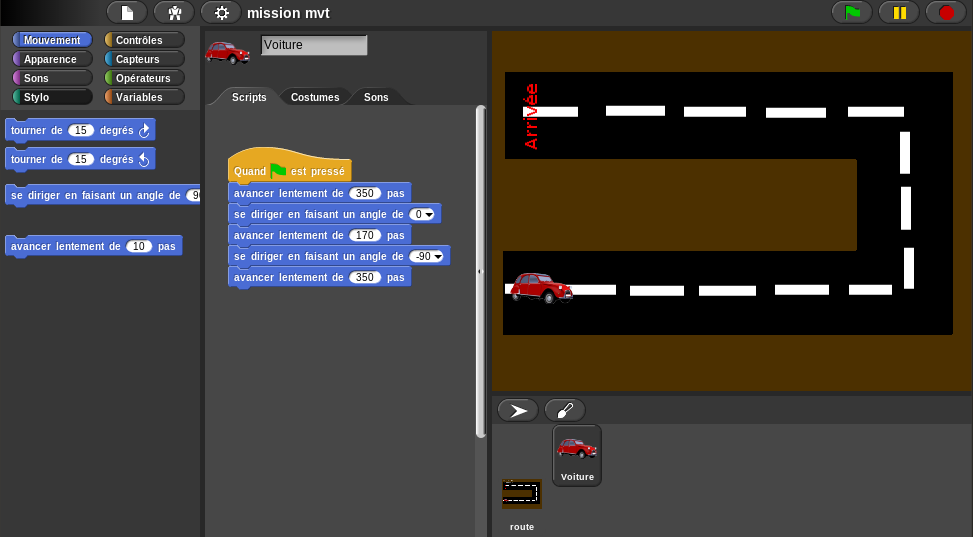
\includegraphics[width=\textwidth]{content/7-solution/1-missions/images/voiture}
    \caption{Mission de la voiture}
    \label{fig:mission-voiture}
  \end{center}
\end{figure}


\subsection{L'hélicoptère}
\label{mission-helicoptere}
Pour cette mission, voir figure \ref{fig:mission-hélicoptère}, les élèves sont aux commandes d'un hélicoptère. Leur but est de faire le tour de la piste. La piste est un ellipsoïde bordée d'herbe. Cette forme ellipsoïde force les étudiants à utiliser des boucles et non un grand nombre de blocs créant une solution particulière. Si l'hélicoptère touche l'herbe, il explose. Sur le contour extérieur de la piste, une bande rouge et une bande bleue sont dessinées. Le but de cette mission est de tourner dés qu'une de ces deux couleurs est touchée pour éviter l'explosion de l'hélicoptère. Comme pour la mission précédente, à chaque lancement de script, l'hélicoptère se repositionne à son point de départ.\\

Les concepts introduits par cette mission sont :
\begin{itemize}
\item les boucles, particulièrement le \texttt{boucler infiniment} ;
\item la gestion des collisions grâce aux capteurs de couleurs ;
\item la division en sous processus (un pour avancer, un pour la collision rouge et un pour la bleue).
\end{itemize}

\begin{figure}
  \begin{center}
    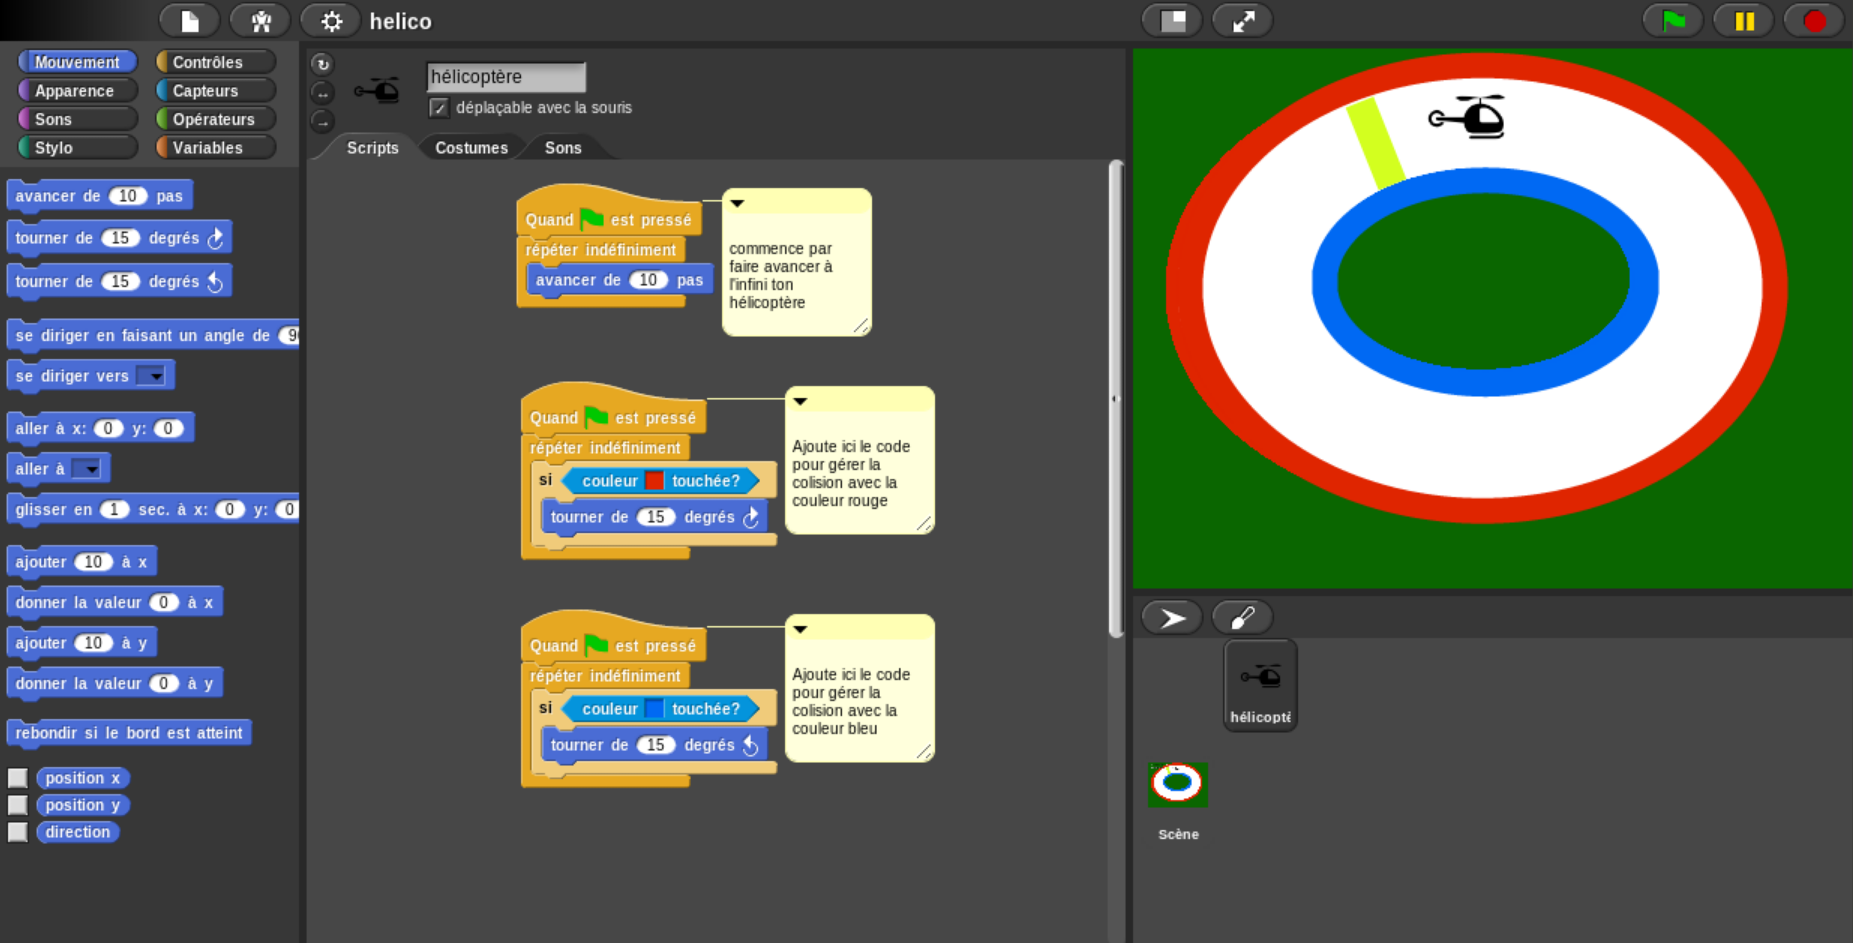
\includegraphics[width=\textwidth]{content/7-solution/1-missions/images/helicoptere}
    \caption{Mission de l'hélicoptère}
    \label{fig:mission-hélicoptère}
  \end{center}
\end{figure}

\subsection{Soyons courtois}
\label{mission-courtois}
Dans cette dernière mission de préparation, voir figure \ref{fig:courtois}, les participants dirigent un personnage qui croise d'autres personnages. Ces derniers disent bonjour à chaque fois qu'ils croisent quelqu'un. Le but de la mission est que le personnage de l'élève réponde.

Les concepts introduits par cette mission sont :
\begin{itemize}
\item la gestion des collisions grâce au capteur sur leur personnage ;
\item la division en sous processus (un pour chaque personne) ;
\item l'introduction à l'interactivité de l'interface, leur personnage est déplaçable à l'aide des flèches du clavier. ;
\item la gestion des dialogues et de l'affichage de textes.
\end{itemize}

\begin{figure}
  \begin{center}
    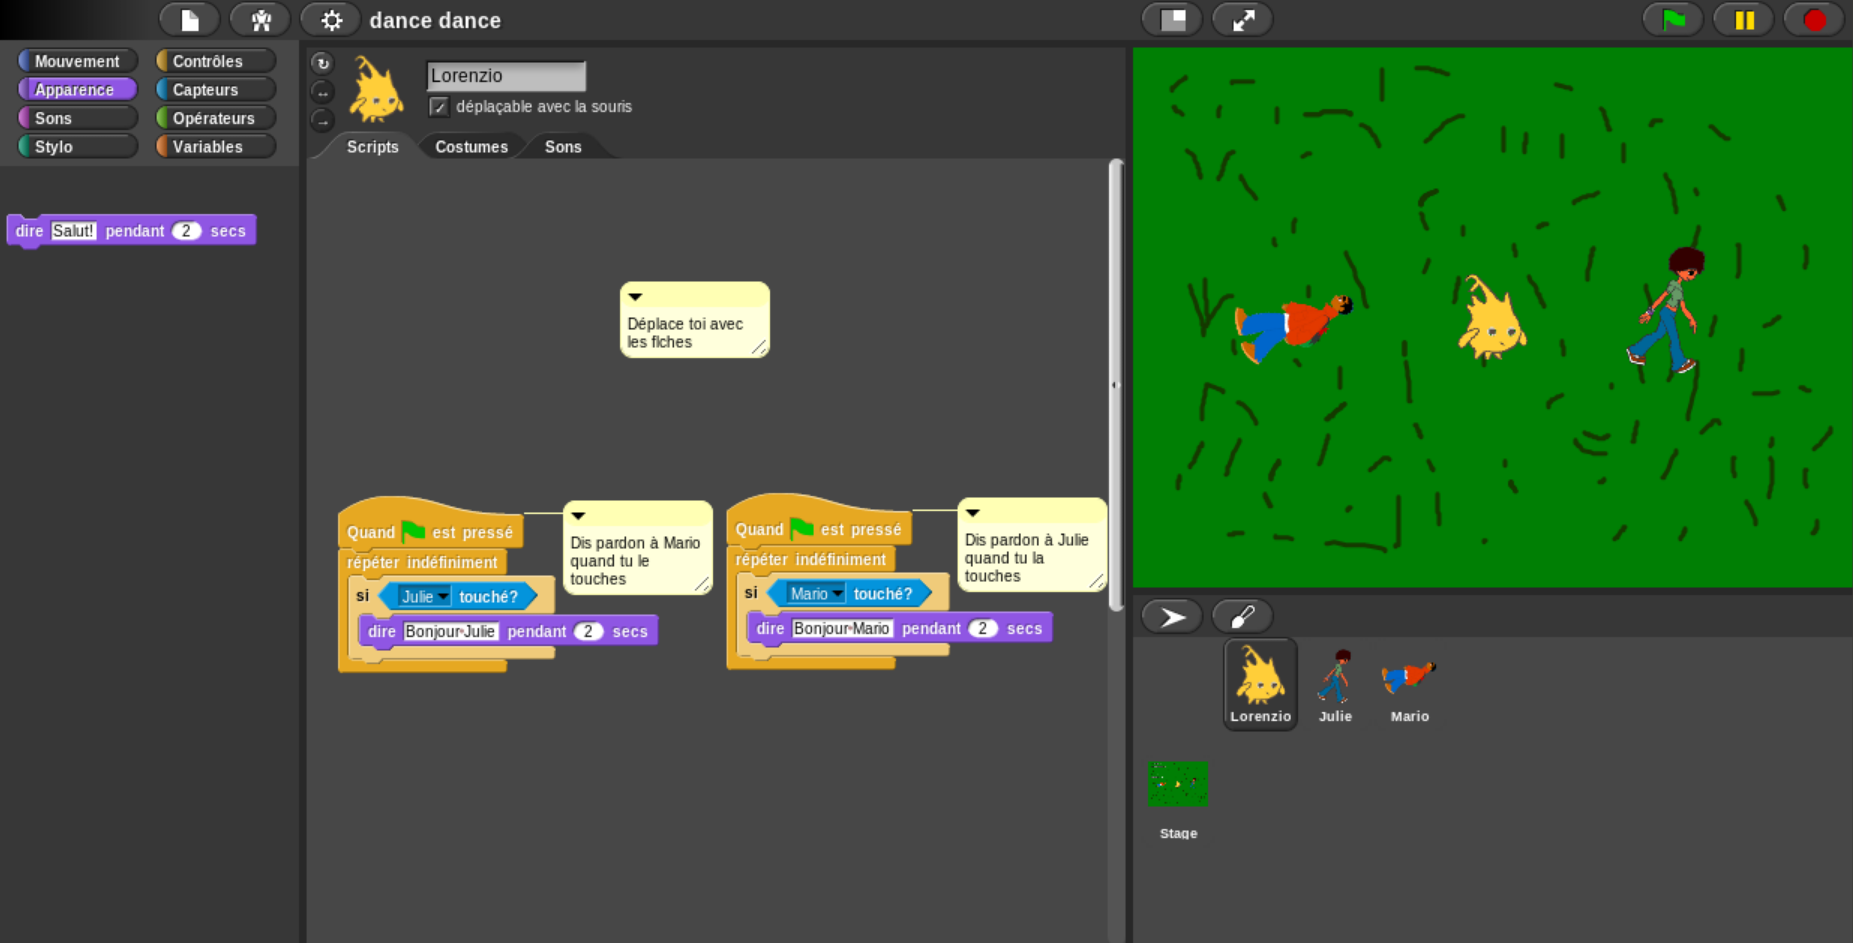
\includegraphics[width=\textwidth]{content/7-solution/1-missions/images/courtois}
    \caption{Mission de soyons courtois}
    \label{fig:courtois}
  \end{center}
\end{figure}

\subsection{Tu ne m'attraperas jamais}
\label{chien-chat}
Cette mission est la dernière de la série et a pour but de mettre ensemble tous les concepts vus dans les missions de préparations. Dans cette mission, les étudiants doivent faire en sorte d'avoir deux personnages et de pouvoir les déplacer séparément à l'aide des touches. Le chien doit courir après le chat. Sur base de propositions faites, les participants déterminent librement l'application exacte des effets de la poursuite. Par exemple, si le chat est touché par le chien, il crie.\\

Cette mission reprend les concepts vus dans les missions de préparation auxquels elle ajoute :
\begin{itemize}
\item modification de l'interface de jeu ;
\item l'activation d'un script sur un événement (déplacements) ;
\end{itemize}

En ce qui concerne les déplacements, ils sont déjà présents dans la mission précédente mais à l'état passif. Les étudiants ne font que l'utiliser. Dans cette mission, ils doivent coder eux-même le fait de pouvoir déplacer leur personnage à l'aide du clavier. Cette application approfondie du concept de déplacement fixe un concept important pour utiliser une interaction avec le clavier.

%analyse mission voiture, cela à permis de prendre en main les entrées des blocs. Au début, beaucoup prennent 3 blocs avancer de 10 pas pour faire 30 pas au lieu de changer la valeur du 10 en 30.
